AMIGO (Autonomous Mate for Intelligent Operations, see Fig.~\ref{fig:amigo}) has competed in RoboCup@Home since 2011. Its design is based on a Middle Size League soccer robot, equipped with two Philips Experimental Robotic Arms mounted on an extensible upper body. Based on our experiences with AMIGO, SERGIO (Second Edition Robot for Generic Indoor Operations, see Fig.~\ref{fig:sergio}) has been developed. The main differences with AMIGO are the use of Mecanum wheels which are compliantly suspended, the torso with two degrees of freedom and the modular setup. The core specifications of AMIGO and SERGIO can be found in Table~\ref{tab:hardwarespec}. More details about the robots can be found on the Robotic Open Platform\footnote{\texttt{http://www.roboticopenplatform.org/}}, where all CAD drawings, electrical schemes and CAD files are published. 
\begin{table}[H]
    \begin{center}
    \caption{Core specifications of AMIGO and SERGIO}
    \label{tab:hardwarespec}
    \renewcommand{\arraystretch}{1.0}
    \setlength{\tabcolsep}{5pt}
        \begin{tabular}{p{0.2\textwidth} p{0.4\textwidth} p{0.4\textwidth}}
            \toprule
            & AMIGO & SERGIO\\
            \midrule
            Name & Autonomous Mate for IntelliGent Operations & Second Edition Robot for Generic Indoor Operations \\
            Base & Fully holonomic omni-wheel platform based on a soccer robot & Fully holonomic Mecanum wheel platform with independent wheel suspension system\\
            Torso & 1 vertical DoF using a ball screw & 1 nearly vertical DoF using a coupled ankle and knee joint, 1 rotational hip joint\\
            Manipulators & 2 7-DoF Philips Experimental Robotic Arms & 2 7-DoF custom arms \\
            Neck & Pan-tilt unit using two Dynamixel RX-28 servo actuators & Pan-tilt unit using two Dynamixel RX-64 servo actuators \\
            Head & Kinect for XBox 360 & Kinect for XBox 360 \\
            External devices & Wireless emergency button & Wireless emergency button \\
            Dimensions & Diameter: $0.75\ \mathrm{m}$, height: $\pm1.5\ \mathrm{m}$ & Base: $0.7\ \mathrm{m}\times0.6\ \mathrm{m}$, height: $\pm1.65\ \mathrm{m}$\\
            Weight & $\pm70\ \mathrm{kg}$ & $\pm70\ \mathrm{kg}$ \\
            Additional sensors & Hokuyo UTM-30LX laser range finder on base and torso & Hokuyo UTM-30LX laser range finder on base and torso (tilting) \\
            Microphone & R{\O}DE Videomic & R{\O}DE Videomic Pro\\
            Batteries & $4\times$ Makita $24\ \mathrm{V},\ 3.3\ \mathrm{Ah}$ & $4\times$ Makita $24\ \mathrm{V},\ 3.3\ \mathrm{Ah}$\\
            Computers & $4\times$ AOpen Mini PC with Core-i7 processor and $8\ \mathrm{Gb}$ RAM & $3\times$ Gigabyte mini ITX board with Core-i7 processor and 	$16\ \mathrm{Gb}$ RAM \\
            \bottomrule
        \end{tabular}
    \end{center}
\end{table}
\begin{figure}[ht]
	\begin{minipage}[t]{0.48\textwidth}
		\centering
		%        \includegraphics[height = 6cm, bb = 0 0 590 812]{Figures/AMIGO_BvOF_Cropped.jpg}
		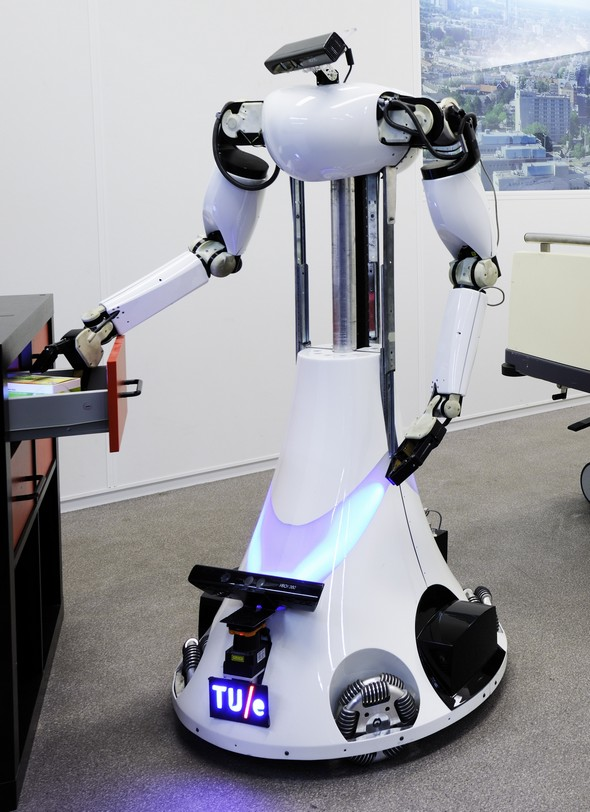
\includegraphics[height = 5.0cm]{Figures/amigo.jpg}
		\caption{The AMIGO robot.}
		\label{fig:amigo}
	\end{minipage}
	\hfill
	\begin{minipage}[t]{0.48\textwidth}
		\centering
		%        \includegraphics[height = 6cm, bb = 0 0 687 1069]{Figures/Total_assy_v1.png}
		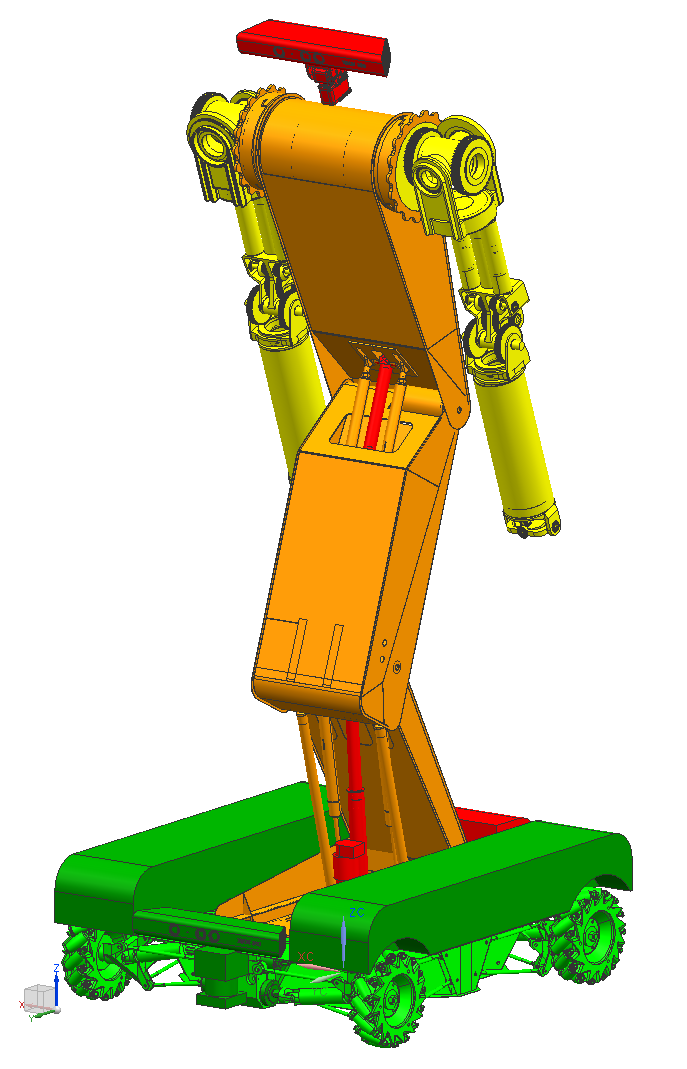
\includegraphics[height = 5.0cm]{Figures/sergio.png}
		\caption{CAD drawing of SERGIO.}
		\label{fig:sergio}
	\end{minipage}
\end{figure}